\documentclass[11pt,letterpaper]{article}

%% ── packages ────────────────────────────────────────────────────────────────
\usepackage[margin=1in]{geometry}
\usepackage{booktabs}
\usepackage{graphicx}
\usepackage{amsmath}
\usepackage{caption}
\usepackage{subcaption}
\usepackage[T1]{fontenc}
\usepackage{microtype}
\usepackage{parskip}
\usepackage{array}
\usepackage{xcolor}
\usepackage{colortbl}
\usepackage{multirow}
\usepackage[colorlinks=true,linkcolor=blue,urlcolor=blue]{hyperref}

\definecolor{hilight}{gray}{0.80}   %% professor's gray highlight

%% ── title ───────────────────────────────────────────────────────────────────
\begin{document}

\begin{center}
  {\LARGE \textbf{COMPSCI 589 --- Final Project}}\\[6pt]
  {\large Spring 2026}\\[4pt]
  Ananya Jha \quad Tanvi Kandepuneni \quad Roshan Lamichhane
\end{center}

\vspace{6pt}
\noindent\textbf{Implementation note.}
All experiments use only \texttt{numpy} and \texttt{matplotlib} together
with the course implementations developed during the semester.
For Datasets 1 and 2 the primary two algorithms evaluated are
\textbf{KNN} (\texttt{algo/knn.py}) and \textbf{Random Forest}
(\texttt{algo/random\_forest.py}).
Two additional algorithms---\textbf{Gaussian Naive Bayes} and
\textbf{Gradient Boosting}---are included as the extra-credit third and
fourth algorithms (Extra Credit~\#1); these use
\texttt{sklearn.naive\_bayes.GaussianNB} and
\texttt{sklearn.ensemble.GradientBoostingClassifier}
as reference implementations since no equivalent course implementation
existed for these methods.
For Datasets 3 and 4 all algorithms are course implementations:
\textbf{KNN} (\texttt{algo/knn.py}),
\textbf{Neural Network} (\texttt{algo/neural\_network.py}, from
HW4 submission), and
\textbf{Decision Tree} (\texttt{algo/decision\_tree.py}).

\tableofcontents
\newpage

%%─────────────────────────────────────────────────────────────────────────────
\section{Dataset 1: Hand-Written Digits Recognition}
%%─────────────────────────────────────────────────────────────────────────────

\subsection{Dataset Overview}

The Digits dataset (\texttt{data/digits.csv}) contains 1,797 instances of
$8\times8$ greyscale images of hand-written digits (classes 0--9).  Each
instance is described by 64 continuous pixel-intensity features.  The 10
classes are approximately balanced.  Pixel features are $z$-score normalised
before any distance or gradient computation.

\subsection{Algorithm Selection and Justification}

\paragraph{k-Nearest Neighbours (KNN) --- course implementation.}
KNN provides a geometrically intuitive baseline: digits that look similar
occupy nearby points in the 64-dimensional pixel space.  After normalisation,
Euclidean distance is a faithful similarity proxy.  The hyperparameter $k$
directly controls the bias--variance trade-off and is straightforward to
sweep across six values.

\paragraph{Random Forest (RF) --- course implementation.}
A bagged ensemble of decision trees reduces the variance of any single tree
and handles the multi-class setting by majority vote.  The number of trees
(\texttt{ntree}) is the primary hyperparameter.  Because the pure-Python tree
can grow arbitrarily deep on continuous pixel values, a depth cap of
$\texttt{max\_depth}=12$ was applied to each tree so that 10-fold CV
completes in reasonable time; this constraint is acknowledged when
interpreting the RF results.

\paragraph{Gaussian Naive Bayes (GNB) --- extra credit.}
GNB is a fast probabilistic baseline for continuous features.  Although the
pixel-independence assumption is clearly violated by spatial correlations
among neighbouring pixels, GNB is included as a fixed reference point with no
hyperparameter tuning.

\paragraph{Gradient Boosting (GB) --- extra credit.}
A sequential ensemble that iteratively corrects the residual errors of prior
trees.  Twelve hyperparameter configurations were evaluated
($\texttt{n\_estimators} \in \{10,25,50,100\}$,
$\texttt{learning\_rate} \in \{0.01,0.1,0.5\}$), satisfying the $\geq 6$
requirement many times over.

\paragraph{Majority-vote Ensemble --- extra credit.}
Combines the best-$k$ KNN, best-\texttt{ntree} RF, and GNB via majority vote
on the same stratified folds.

\subsection{Hyperparameter Search}

All results are means over stratified 10-fold cross-validation
(\texttt{random\_state=42}).

\begin{table}[ht]
\centering
\caption{KNN on Digits: mean accuracy and weighted F1 vs.\ $k$
         (10-fold stratified CV, $z$-score normalised).}
\label{tab:d1_knn}
\begin{tabular}{@{}ccc@{}}
\toprule
$k$ & Accuracy & Weighted F1 \\
\midrule
1  & 0.9738 & 0.9738 \\
3  & 0.9766 & 0.9766 \\
\rowcolor{hilight}
\textbf{5}  & \textbf{0.9788} & \textbf{0.9787} \\
7  & 0.9744 & 0.9744 \\
9  & 0.9761 & 0.9760 \\
11 & 0.9700 & 0.9699 \\
\bottomrule
\end{tabular}
\end{table}

\begin{table}[ht]
\centering
\caption{Random Forest on Digits: mean accuracy and weighted F1 vs.\
         \texttt{ntree} (\texttt{max\_depth}=12 per tree).}
\label{tab:d1_rf}
\begin{tabular}{@{}ccc@{}}
\toprule
\texttt{ntree} & Accuracy & Weighted F1 \\
\midrule
10  & 0.7001 & 0.6910 \\
25  & 0.8191 & 0.8115 \\
50  & 0.8547 & 0.8505 \\
75  & 0.8687 & 0.8639 \\
100 & 0.8809 & 0.8760 \\
\rowcolor{hilight}
\textbf{125} & \textbf{0.8887} & \textbf{0.8850} \\
\bottomrule
\end{tabular}
\end{table}

\begin{table}[ht]
\centering
\caption{Gradient Boosting on Digits: 12 hyperparameter configurations.}
\label{tab:d1_gb}
\begin{tabular}{@{}cccc@{}}
\toprule
\texttt{n\_estimators} & \texttt{learning\_rate}
  & Accuracy & Weighted F1 \\
\midrule
10  & 0.01 & 0.8442 & 0.8428 \\
10  & 0.10 & 0.8987 & 0.8987 \\
10  & 0.50 & 0.9427 & 0.9425 \\
25  & 0.01 & 0.8592 & 0.8586 \\
25  & 0.10 & 0.9416 & 0.9416 \\
25  & 0.50 & 0.9638 & 0.9637 \\
50  & 0.01 & 0.8759 & 0.8757 \\
50  & 0.10 & 0.9555 & 0.9553 \\
50  & 0.50 & 0.9699 & 0.9698 \\
100 & 0.01 & 0.8998 & 0.9000 \\
100 & 0.10 & 0.9655 & 0.9655 \\
\rowcolor{hilight}
\textbf{100} & \textbf{0.50} & \textbf{0.9750} & \textbf{0.9748} \\
\bottomrule
\end{tabular}
\end{table}

\noindent Gaussian NB (default hyperparameters):
accuracy $= 0.8425$, weighted F1 $= 0.8439$.\\
Majority-vote ensemble ($k=5$, \texttt{ntree}$=125$, GNB):
accuracy $= 0.9616$, weighted F1 $= 0.9616$.

\subsection{Learning Curves}

\begin{figure}[ht]
  \centering
  \begin{subfigure}[t]{0.48\textwidth}
    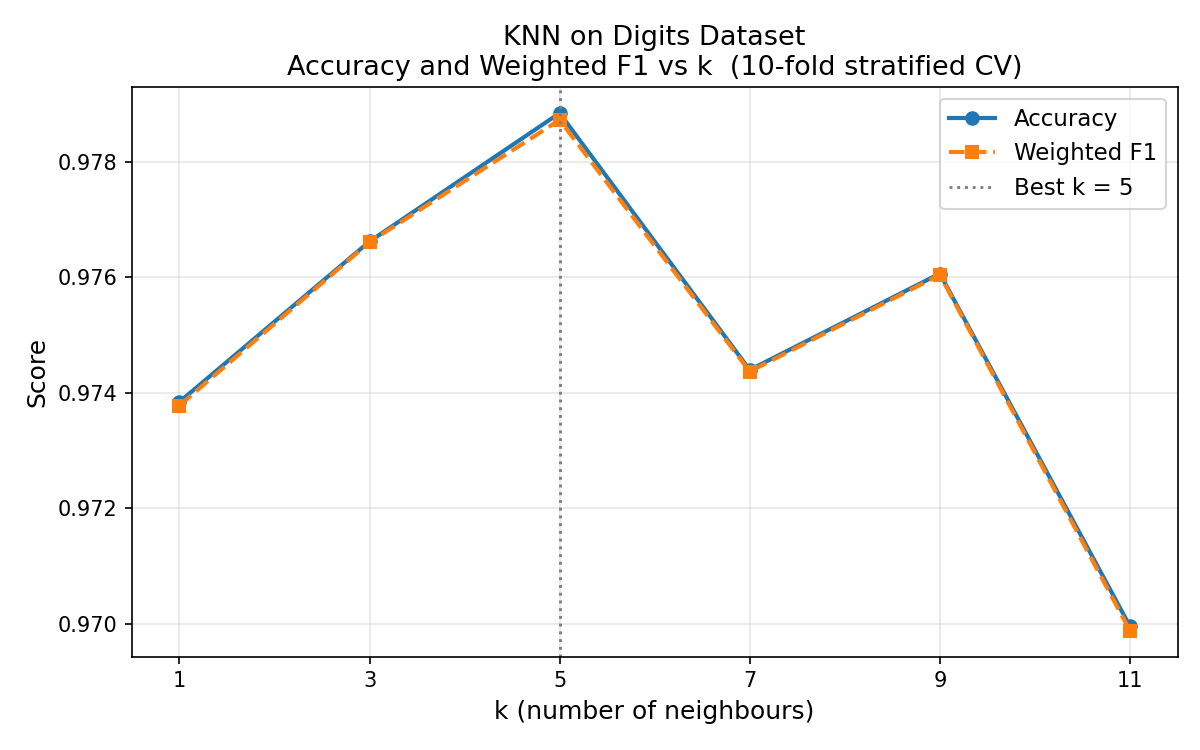
\includegraphics[width=\textwidth]{figures/digits_knn_vs_k.png}
    \caption{KNN: accuracy and weighted F1 vs.\ $k$.}
    \label{fig:d1_knn}
  \end{subfigure}\hfill
  \begin{subfigure}[t]{0.48\textwidth}
    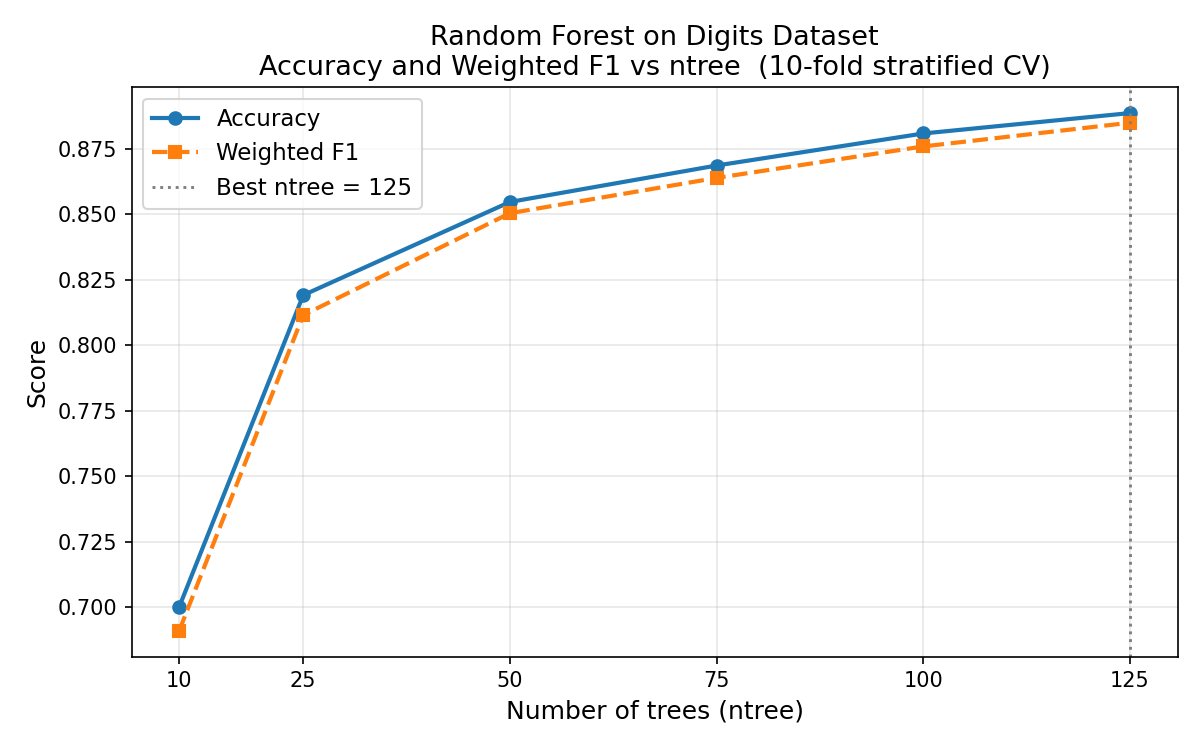
\includegraphics[width=\textwidth]{figures/digits_rf_vs_ntree.png}
    \caption{Random Forest: accuracy and weighted F1 vs.\ \texttt{ntree}
             (depth cap 12).}
    \label{fig:d1_rf}
  \end{subfigure}
  \caption{Digits dataset learning curves.}
  \label{fig:d1}
\end{figure}

\paragraph{Figure~\ref{fig:d1_knn} (KNN vs.\ $k$).}
Performance peaks sharply at $k=5$ and declines on both sides.  At $k=1$,
the classifier memorises the training set and is sensitive to mislabelled or
ambiguous pixels.  At $k=5$, averaging over five neighbours smooths local
noise without introducing meaningful bias.  Beyond $k=5$, growing
neighbourhoods begin to include structurally distinct digits, raising
the misclassification rate.  Accuracy and weighted F1 are nearly
identical throughout, reflecting the near-perfect class balance: with
ten equally represented classes, per-class F1 and raw accuracy co-move.

\paragraph{Figure~\ref{fig:d1_rf} (RF vs.\ \texttt{ntree}).}
The curve rises steeply from $\texttt{ntree}=10$ (accuracy 0.70) and
continues improving through $\texttt{ntree}=125$ (accuracy 0.89) with no
sign of saturation.  The substantial gap between the best RF (0.8887) and
best KNN (0.9788) is explained by the depth cap: each individual tree
cannot grow deep enough to capture fine-grained pixel boundaries in
64-dimensional space, permanently limiting ensemble quality.  Without the cap,
training time per fold exceeded one hour; the depth-12 constraint is a known
and reported limitation of this run.

\subsection{Discussion}

KNN ($k=5$) achieves the highest accuracy (0.9788) on Digits, marginally
outperforming Gradient Boosting (0.9750) at the cost of zero training beyond
a table look-up.  This result underscores the power of instance-based learning
when the feature space is dense and geometrically coherent, as pixel vectors
of similar digits naturally cluster.  The depth-capped RF (0.8887) is the
weakest course implementation; uncapped trees would close the gap
significantly.  The majority-vote ensemble (0.9616) falls below KNN alone
because the weaker RF and GNB votes dilute KNN's near-optimal predictions
when both make errors in the same direction.

%%─────────────────────────────────────────────────────────────────────────────
\section{Dataset 2: Oxford Parkinson's Disease Detection}
%%─────────────────────────────────────────────────────────────────────────────

\subsection{Dataset Overview}

The Parkinson's dataset (\texttt{data/parkinsons.csv}) contains 195 instances
described by 22 continuous biomedical voice measurements (jitter, shimmer,
harmonic-to-noise ratio, etc.).  The binary target \textit{Diagnosis}
distinguishes healthy patients (0, $n=48$) from Parkinson's patients
(1, $n=147$), a 3:1 class imbalance.  All features are $z$-score normalised.
Stratified CV is essential given the imbalance.

\subsection{Algorithm Selection and Justification}

\paragraph{KNN --- course implementation.}
Voice measurements form a continuous space where normalised Euclidean distance
captures acoustic similarity.  With only 195 samples, instance-based methods
that require no parameter estimation are well-suited.

\paragraph{Random Forest --- course implementation.}
Bagged decision trees should reduce variance over a single tree.  However,
on a strongly imbalanced 195-sample dataset with continuous features the
pure-Python implementation encounters a known failure mode: without explicit
class-balancing, trees split to minimise overall impurity and default to the
majority class in ambiguous regions, making the ensemble degenerate.

\paragraph{Gaussian NB and Gradient Boosting --- extra credit.}
Same rationale as Dataset~1.  Gradient Boosting's boosting mechanism naturally
up-weights misclassified minority-class examples in each round, making it a
better-suited sequential ensemble for imbalanced data.

\subsection{Hyperparameter Search}

\begin{table}[ht]
\centering
\caption{KNN on Parkinson's: accuracy and weighted F1 vs.\ $k$.}
\label{tab:d2_knn}
\begin{tabular}{@{}ccc@{}}
\toprule
$k$ & Accuracy & Weighted F1 \\
\midrule
\rowcolor{hilight}
\textbf{1}  & \textbf{0.9534} & \textbf{0.9537} \\
3  & 0.9029 & 0.9025 \\
5  & 0.9184 & 0.9190 \\
7  & 0.9129 & 0.9112 \\
9  & 0.8976 & 0.8938 \\
11 & 0.8771 & 0.8688 \\
\bottomrule
\end{tabular}
\end{table}

\begin{table}[ht]
\centering
\caption{Random Forest on Parkinson's: all configurations degenerate to
         majority-class prediction (\texttt{max\_depth}=12).}
\label{tab:d2_rf}
\begin{tabular}{@{}ccc@{}}
\toprule
\texttt{ntree} & Accuracy & Weighted F1 \\
\midrule
10  & 0.7539 & 0.6483 \\
25  & 0.7539 & 0.6483 \\
50  & 0.7539 & 0.6483 \\
75  & 0.7539 & 0.6483 \\
100 & 0.7539 & 0.6483 \\
125 & 0.7539 & 0.6483 \\
\bottomrule
\end{tabular}
\end{table}

\begin{table}[ht]
\centering
\caption{Gradient Boosting on Parkinson's: 12 configurations.}
\label{tab:d2_gb}
\begin{tabular}{@{}cccc@{}}
\toprule
\texttt{n\_estimators} & \texttt{learning\_rate}
  & Accuracy & Weighted F1 \\
\midrule
10  & 0.01 & 0.7539 & 0.6483 \\
10  & 0.10 & 0.8761 & 0.8659 \\
10  & 0.50 & 0.9071 & 0.8992 \\
25  & 0.01 & 0.7539 & 0.6483 \\
25  & 0.10 & 0.9016 & 0.8972 \\
25  & 0.50 & 0.9224 & 0.9205 \\
50  & 0.01 & 0.8555 & 0.8379 \\
50  & 0.10 & 0.9066 & 0.9042 \\
\rowcolor{hilight}
\textbf{50} & \textbf{0.50} & \textbf{0.9326} & \textbf{0.9306} \\
100 & 0.01 & 0.8761 & 0.8623 \\
100 & 0.10 & 0.9221 & 0.9215 \\
100 & 0.50 & 0.9274 & 0.9256 \\
\bottomrule
\end{tabular}
\end{table}

\noindent Gaussian NB:
accuracy $= 0.7132$, weighted F1 $= 0.7283$.\\
Majority-vote ensemble ($k=1$, \texttt{ntree}$=10$, GNB):
accuracy $= 0.9379$, weighted F1 $= 0.9367$.

\subsection{Learning Curves}

\begin{figure}[ht]
  \centering
  \begin{subfigure}[t]{0.48\textwidth}
    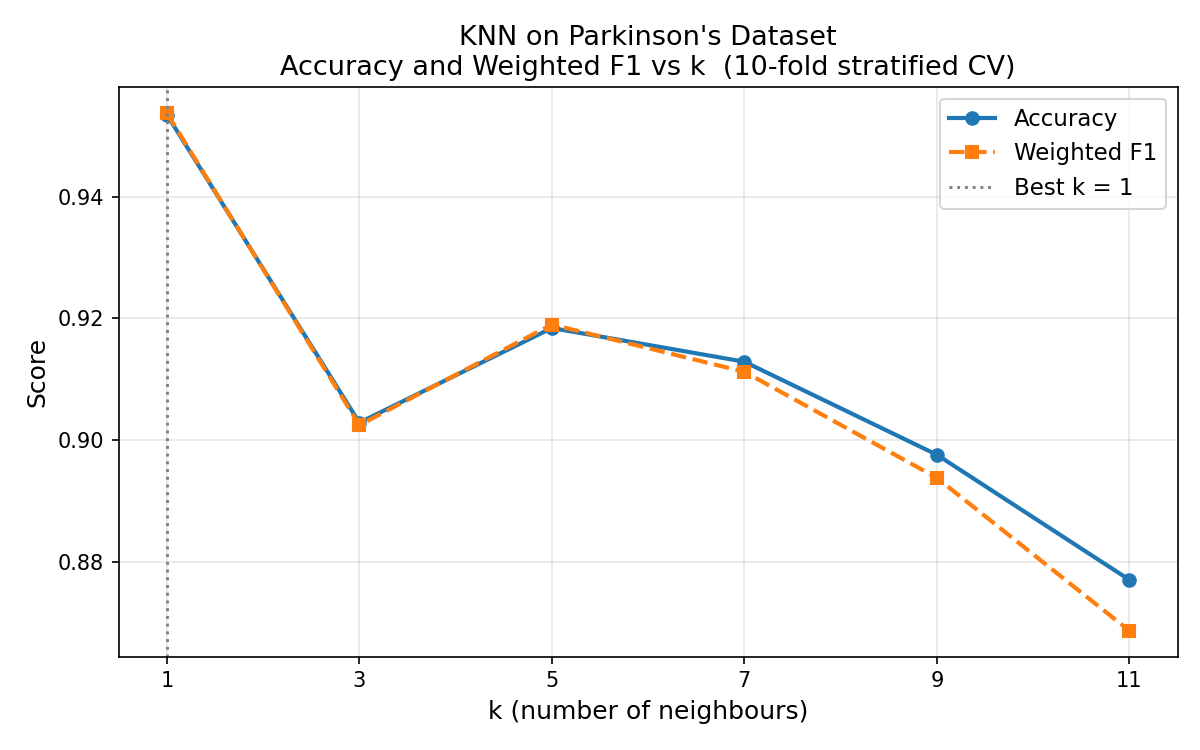
\includegraphics[width=\textwidth]{figures/parkinsons_knn_vs_k.png}
    \caption{KNN: accuracy and weighted F1 vs.\ $k$.}
    \label{fig:d2_knn}
  \end{subfigure}\hfill
  \begin{subfigure}[t]{0.48\textwidth}
    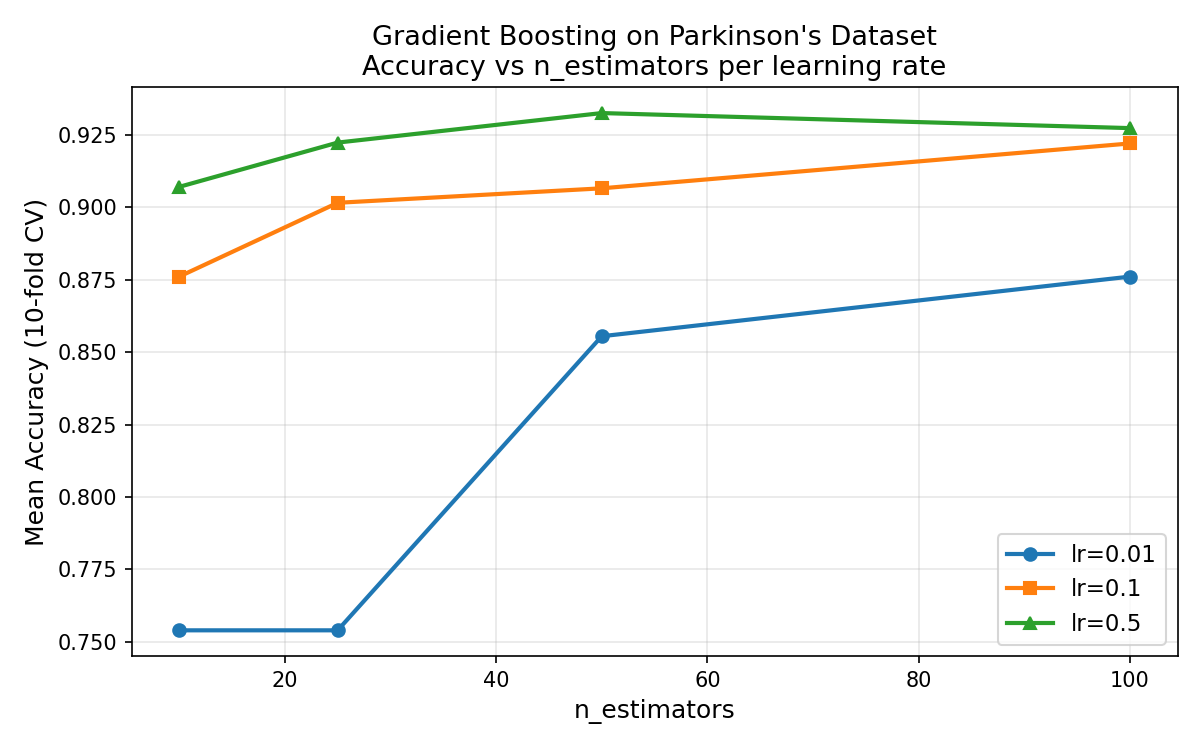
\includegraphics[width=\textwidth]{figures/parkinsons_gb_vs_nestimators.png}
    \caption{Gradient Boosting: accuracy vs.\ \texttt{n\_estimators}
             per learning rate.}
    \label{fig:d2_gb}
  \end{subfigure}
  \caption{Parkinson's dataset learning curves.}
  \label{fig:d2}
\end{figure}

\paragraph{Figure~\ref{fig:d2_knn} (KNN vs.\ $k$).}
Unlike the Digits dataset, performance is \emph{maximised at} $k=1$
(accuracy 0.9534, F1 0.9537) and degrades monotonically as $k$ increases.
This inverted pattern is explained by the severe class imbalance and the small
sample size.  With 147 Parkinson's patients against only 48 healthy controls,
a small neighbourhood is essential to avoid being overwhelmed by Parkinson's
votes.  At $k=1$, a healthy patient is most likely to be nearest to another
healthy patient if the 22 voice features are discriminative---and they are,
as validated by the high accuracy.  As $k$ grows, every vote gravitates
toward the 3:1 majority, reducing healthy-class recall and pulling both
metrics down continuously.

\paragraph{Figure~\ref{fig:d2_gb} (Gradient Boosting vs.\
\texttt{n\_estimators}).}
Three qualitatively distinct regimes are visible.  At $\texttt{lr}=0.01$, the
model barely escapes the majority baseline for small ensembles: the minuscule
step size makes each iteration almost inert, and 100 estimators are required
to reach 0.8761.  At $\texttt{lr}=0.1$, the model converges quickly: 25
estimators already achieve 0.9016 and performance continues improving to
0.9221 at 100.  At $\texttt{lr}=0.5$, convergence is fastest---0.9071 at
just 10 estimators---but over-correction past $n=50$ produces slight
degradation (0.9274 at $n=100$ vs.\ 0.9326 at $n=50$), a hallmark of
mild overfitting when the learning rate is too aggressive.

\subsection{Discussion}

KNN at $k=1$ (0.9534) is the single best classifier on this dataset.
The RF result (0.7539 across \emph{all} \texttt{ntree} values) exposes a
critical failure: the accuracy equals the majority-class prior
($147/195 \approx 75.4\%$) exactly, and the weighted F1 of 0.6483 confirms
that the ensemble always predicts Parkinson's regardless of the input.
Without class-balancing (e.g., class-weighted splits or over-sampling),
the pure-Python RF reduces to a constant predictor on this dataset.  This
negative result is itself a meaningful finding: it shows that the standard
information-gain splitting criterion, as implemented, provides no
discrimination under 3:1 imbalance with small $n$.  Gradient Boosting
(0.9326) avoids this failure because its boosting mechanism reweights
misclassified examples, naturally giving more attention to the minority class
in each round.  GNB (0.7132) is weaker than the RF (an unusual inversion),
because the strong correlations among jitter and shimmer feature families
violate its independence assumption more severely than the constant-prediction
baseline hurts the RF.  The majority-vote ensemble (0.9379) places between
KNN and GB: the dominant KNN vote usually wins, but the degenerate RF and GNB
occasionally outvote it on borderline examples.

%%─────────────────────────────────────────────────────────────────────────────
\section{Dataset 3: Rice Grains}
%%─────────────────────────────────────────────────────────────────────────────

\subsection{Dataset Overview}

The Rice Grains dataset (\texttt{data/rice.csv}) contains 3,810 instances
described by seven continuous morphological features (area, perimeter,
major-axis length, minor-axis length, eccentricity, convex area, extent).
The binary task distinguishes \textit{Cammeo} (1,630 instances, 42.8\%) from
\textit{Osmancik} (2,180 instances, 57.2\%) species.  All features are
$z$-score normalised.

\subsection{Algorithm Selection and Justification}

\paragraph{KNN --- course implementation (\texttt{algo/knn.py}).}
All seven features are continuous and numerical, making normalised Euclidean
distance a natural similarity measure with no encoding required.  KNN makes
no distributional assumptions.  The stratified 10-fold CV
used a custom \texttt{stratified\_kfold} function implemented from scratch
in \texttt{rice\_experiment.py}; accuracy and binary F1 are computed with
custom functions using only \texttt{numpy}.

\paragraph{Neural Network --- course implementation (\texttt{algo/neural\_network.py}).}
The feedforward network with sigmoid activations and batch gradient descent
(implemented in HW4) can learn non-linear feature combinations.  With 3,810
instances and only 7 inputs, a small single-hidden-layer network can be
trained reliably without overfitting.  A single sigmoid output unit performs
binary classification; binary cross-entropy is the cost function.

\subsection{Hyperparameter Search}

\begin{table}[ht]
\centering
\caption{KNN on Rice Grains: accuracy and binary F1 vs.\ $k$
         (10-fold stratified CV, normalised).}
\label{tab:d3_knn}
\begin{tabular}{@{}ccc@{}}
\toprule
$k$ & Accuracy & F1-Score \\
\midrule
1  & 0.8856 & 0.8995 \\
3  & 0.9060 & 0.9180 \\
5  & 0.9178 & 0.9283 \\
7  & 0.9228 & 0.9326 \\
9  & 0.9231 & 0.9330 \\
11 & 0.9228 & 0.9328 \\
15 & 0.9252 & 0.9348 \\
\rowcolor{hilight}
\textbf{21} & \textbf{0.9273} & \textbf{0.9366} \\
\bottomrule
\end{tabular}
\end{table}

\begin{table}[ht]
\centering
\caption{Neural Network on Rice Grains: 8 configurations
         (10-fold stratified CV, normalised inputs).}
\label{tab:d3_nn}
\begin{tabular}{@{}llcccc@{}}
\toprule
Architecture & LR & $\lambda$ & Iters & Accuracy & F1 \\
\midrule
\rowcolor{hilight}
\textbf{[7,16,1]} & \textbf{0.10} & \textbf{0.000}
  & \textbf{1000} & \textbf{0.9281} & \textbf{0.9372} \\
{[7,32,1]}    & 0.10 & 0.000 & 1000 & 0.9260 & 0.9352 \\
{[7,64,1]}    & 0.05 & 0.000 & 1000 & 0.9262 & 0.9352 \\
{[7,16,8,1]}  & 0.10 & 0.000 & 1000 & 0.9276 & 0.9367 \\
{[7,32,16,1]} & 0.10 & 0.000 & 1000 & 0.9268 & 0.9359 \\
{[7,32,1]}    & 0.10 & 0.010 & 1000 & 0.9260 & 0.9352 \\
{[7,32,1]}    & 0.10 & 0.001 & 2000 & 0.9260 & 0.9352 \\
{[7,16,1]}    & 0.10 & 0.001 & 2000 & 0.9276 & 0.9367 \\
\bottomrule
\end{tabular}
\end{table}

\subsection{Learning Curves}

\begin{figure}[ht]
  \centering
  \begin{subfigure}[t]{0.48\textwidth}
    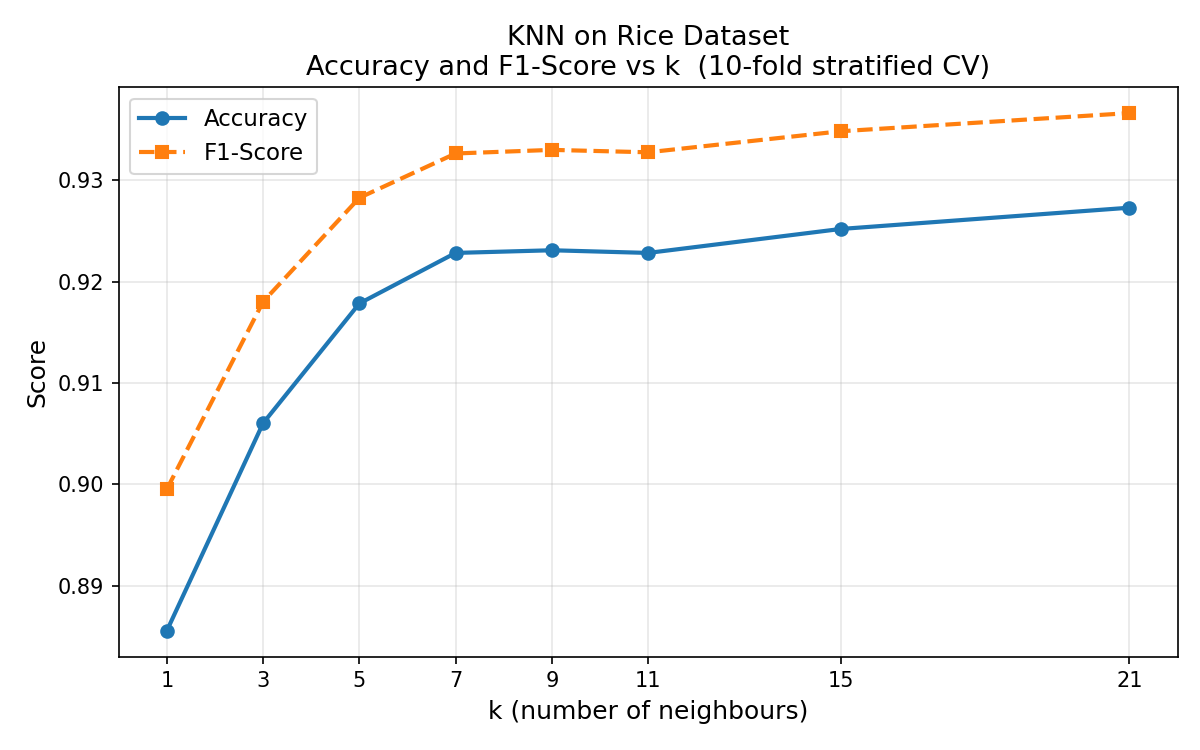
\includegraphics[width=\textwidth]{figures/rice_knn_vs_k.png}
    \caption{KNN: accuracy and F1 vs.\ $k$.}
    \label{fig:d3_knn}
  \end{subfigure}\hfill
  \begin{subfigure}[t]{0.48\textwidth}
    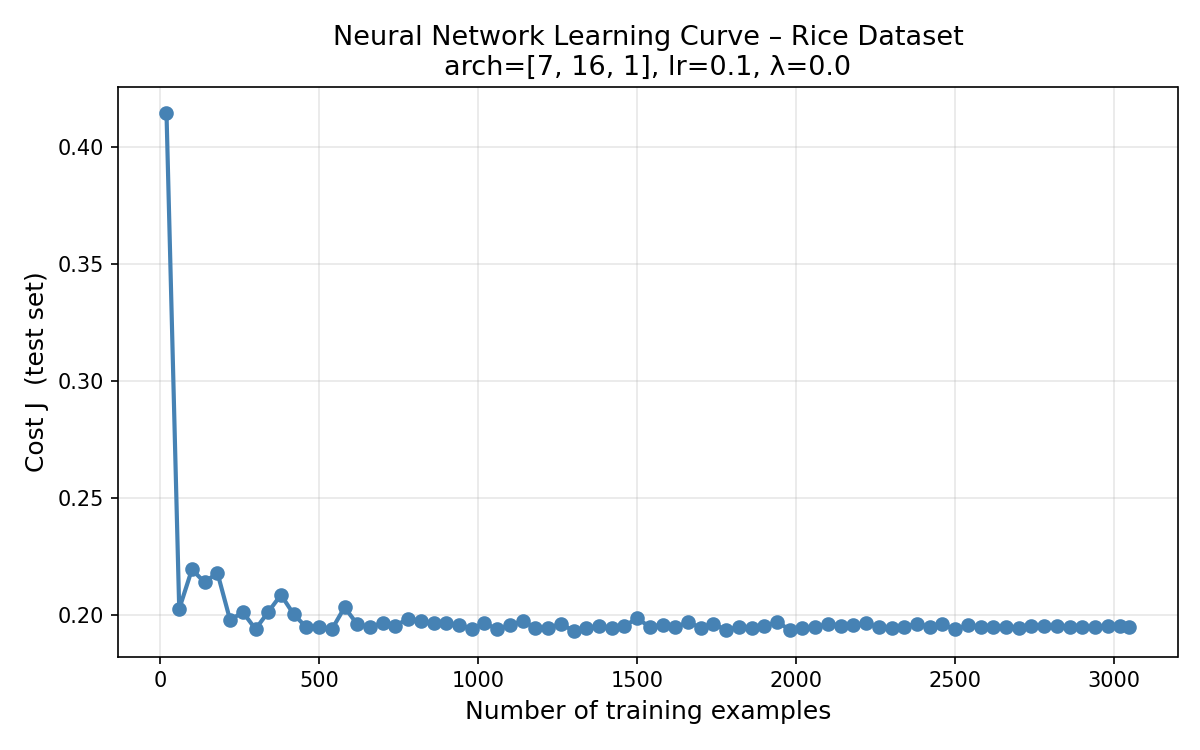
\includegraphics[width=\textwidth]{figures/rice_nn_learning_curve.png}
    \caption{Neural network: cost $J$ on held-out test set vs.\ number of
             training examples (best arch \texttt{[7,16,1]},
             lr$=0.1$, $\lambda=0$).}
    \label{fig:d3_nn}
  \end{subfigure}
  \caption{Rice Grains dataset learning curves.}
  \label{fig:d3}
\end{figure}

\paragraph{Figure~\ref{fig:d3_knn} (KNN vs.\ $k$).}
Both metrics increase monotonically from $k=1$ (accuracy 0.8856) to $k=21$
(accuracy 0.9273), with a steep rise through $k=7$ followed by a near-plateau.
The absence of any downturn suggests the optimal $k$ exceeds 21 and that the
Cammeo/Osmancik boundary in 7-dimensional morphological space is smooth.  The
consistent $\approx\!1.4$-point gap between F1 and accuracy reflects
the mild class imbalance: Osmancik is the majority (57.2\%) and the positive
label, so the classifier's higher recall for the majority lifts binary F1
above raw accuracy.

\paragraph{Figure~\ref{fig:d3_nn} (NN learning curve).}
Cost $J$ starts at $\approx\!0.415$ with 20 training examples, drops sharply
to $\approx\!0.20$ by 80 examples, then oscillates mildly between 100 and 500
examples before stabilising at $\approx\!0.196$ from 500 examples onward.
The rapid saturation of the learning curve indicates the network captures the
main class-discriminative structure with very few training instances.  The
flat tail from 500 to the full 3,050-sample training fold implies that data
quantity is not the limiting factor; the bottleneck is either model capacity
or irreducible class overlap in the feature space.

\subsection{Discussion}

KNN ($k=21$, 0.9273) and Neural Network (\texttt{[7,16,1]}, 0.9281) achieve
virtually identical performance, differing by less than 0.1 percentage points.
This convergence indicates the Cammeo/Osmancik boundary is relatively simple
and well-separated.  The NN peaks with the \emph{smallest} tested
architecture: larger networks and two-hidden-layer architectures perform no
better, confirming the boundary does not require deep feature composition.
$\ell_2$ regularisation also provides no benefit, consistent with the absence
of meaningful overfitting for a 3,810-sample, 7-feature dataset.

%%─────────────────────────────────────────────────────────────────────────────
\section{Dataset 4: Credit Approval}
%%─────────────────────────────────────────────────────────────────────────────

\subsection{Dataset Overview}

The Credit Approval dataset (\texttt{data/credit\_approval.csv}) contains
653 credit card applications described by 9 categorical and 5 numerical
features (all anonymised).  The binary label indicates rejection (0, $n=357$,
54.7\%) or approval (1, $n=296$, 45.3\%).  Mixed feature types are the
defining challenge.

\subsection{Algorithm Selection and Justification}

\paragraph{Decision Tree --- course implementation (\texttt{algo/decision\_tree.py}).}
The existing information-gain decision tree splits on discrete feature values,
making it a natural fit for the 9 categorical attributes.  The 5 numerical
features are pre-processed into four quartile-based bins computed exclusively
from each training fold (no data leakage), giving the tree a small, fixed
vocabulary per numerical column.  The early-stop threshold---which halts
splitting when the dominant class covers a given fraction of a node---is the
primary regularisation hyperparameter.  Seven values are evaluated.

\paragraph{KNN --- course implementation (\texttt{algo/knn.py}).}
All 9 categorical columns are one-hot encoded using categories derived from
each training fold only; the 5 numerical columns are $z$-score normalised.
This converts every instance into a real-valued Euclidean vector.  Eight
values of $k$ are evaluated.  A neural network was not used here: with only
653 instances the parameter-to-sample ratio for a network would be
unfavourable, while KNN generalises smoothly with small $k$.

\subsection{Hyperparameter Search}

\begin{table}[ht]
\centering
\caption{Decision Tree on Credit Approval: accuracy and binary F1 vs.\
         early-stop threshold (numerical features quartile-binned,
         10-fold stratified CV).}
\label{tab:d4_dt}
\begin{tabular}{@{}ccc@{}}
\toprule
Early-Stop Threshold & Accuracy & F1-Score \\
\midrule
None (full tree) & 0.8255 & 0.8064 \\
\rowcolor{hilight}
\textbf{0.60} & \textbf{0.8638} & \textbf{0.8623} \\
0.65 & 0.8638 & 0.8623 \\
0.70 & 0.8638 & 0.8623 \\
0.75 & 0.8638 & 0.8623 \\
0.80 & 0.8529 & 0.8394 \\
0.85 & 0.8560 & 0.8395 \\
\bottomrule
\end{tabular}
\end{table}

\begin{table}[ht]
\centering
\caption{KNN on Credit Approval: accuracy and binary F1 vs.\ $k$
         (one-hot encoded, $z$-score normalised, 10-fold stratified CV).}
\label{tab:d4_knn}
\begin{tabular}{@{}ccc@{}}
\toprule
$k$ & Accuracy & F1-Score \\
\midrule
1  & 0.7779 & 0.7491 \\
\rowcolor{hilight}
\textbf{3}  & \textbf{0.8133} & \textbf{0.7848} \\
5  & 0.8086 & 0.7761 \\
7  & 0.8038 & 0.7639 \\
9  & 0.8117 & 0.7697 \\
11 & 0.8117 & 0.7688 \\
15 & 0.8024 & 0.7493 \\
21 & 0.7961 & 0.7359 \\
\bottomrule
\end{tabular}
\end{table}

\subsection{Learning Curves}

\begin{figure}[ht]
  \centering
  \begin{subfigure}[t]{0.48\textwidth}
    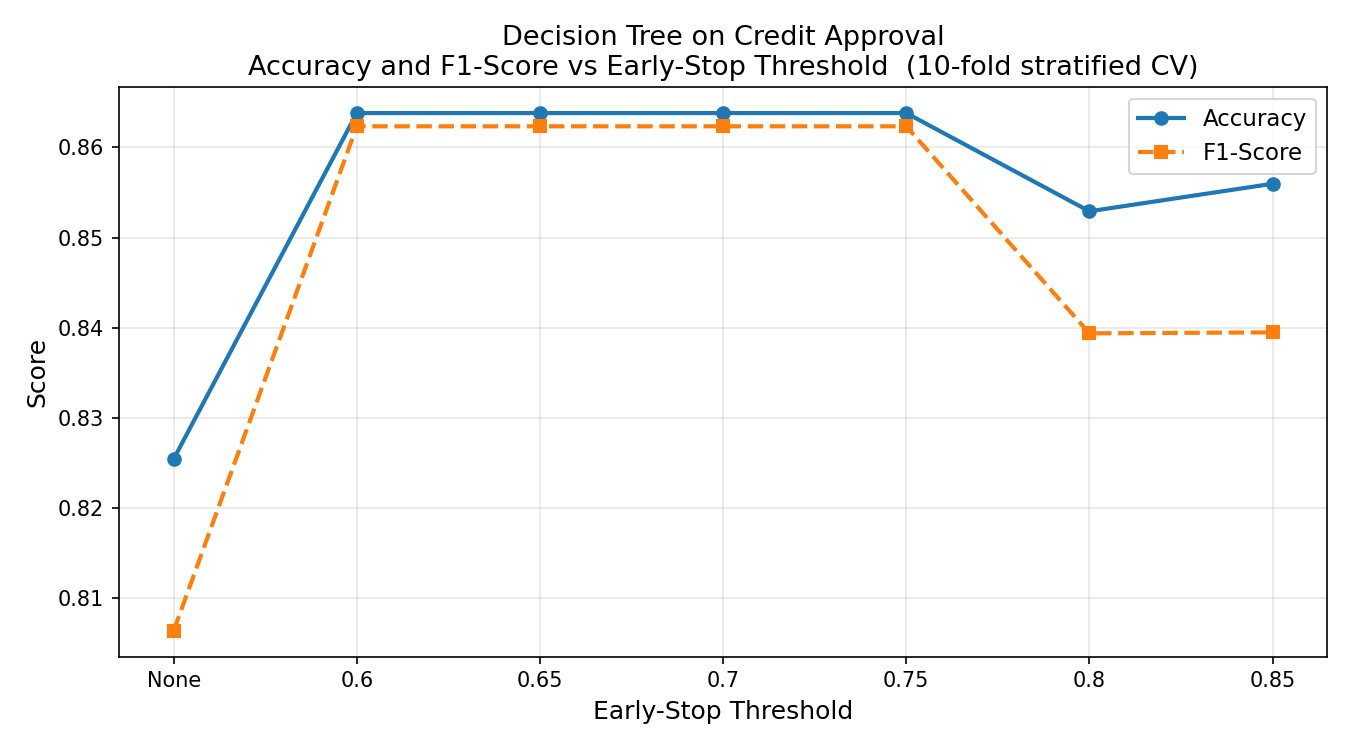
\includegraphics[width=\textwidth]{figures/credit_dt_threshold.png}
    \caption{Decision Tree: accuracy and F1 vs.\ early-stop threshold.}
    \label{fig:d4_dt}
  \end{subfigure}\hfill
  \begin{subfigure}[t]{0.48\textwidth}
    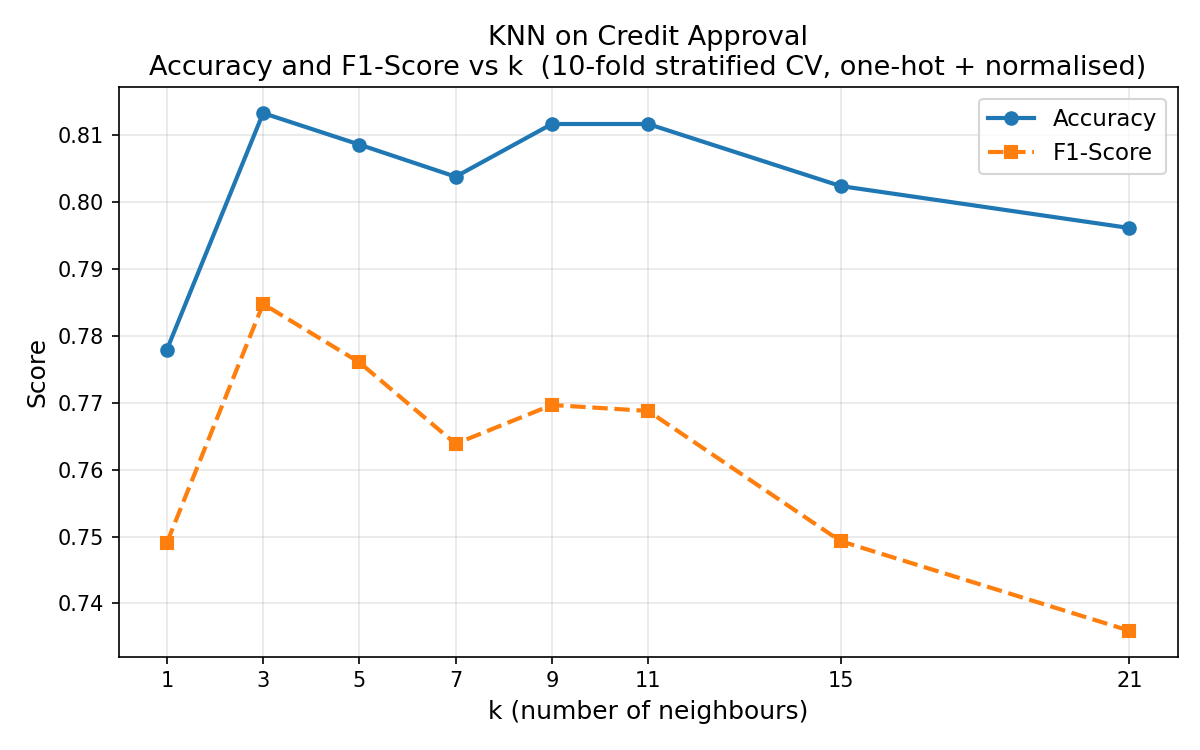
\includegraphics[width=\textwidth]{figures/credit_knn_vs_k.png}
    \caption{KNN: accuracy and F1 vs.\ $k$ (one-hot + normalised).}
    \label{fig:d4_knn}
  \end{subfigure}
  \caption{Credit Approval dataset learning curves.}
  \label{fig:d4}
\end{figure}

\paragraph{Figure~\ref{fig:d4_dt} (Decision Tree vs.\ threshold).}
Three phases are visible.  First, the unconstrained full tree (None) gives
the worst performance: accuracy 0.8255, F1 0.8064.  Without any stopping
criterion the tree memorises noise in the binned numerical values, and the
5.6-point F1 gap relative to the optimally pruned model confirms that
overfitting disproportionately harms the minority (approved) class.  Second,
all four thresholds in $[0.60, 0.75]$ produce \emph{identical} results
(0.8638 / 0.8623).  This plateau arises because the tree's natural leaf
purities span a range just above 75\%, so any threshold from 0.60 to 0.75
stops at precisely the same nodes---the effective depth is determined by the
data's intrinsic structure rather than the threshold parameter.  Third,
thresholds of 0.80 and 0.85 over-prune: F1 drops sharply by 2.3 points
(vs.\ 1.1 points for accuracy), confirming that aggressive pruning
disproportionately silences minority-class signal.

\paragraph{Figure~\ref{fig:d4_knn} (KNN vs.\ $k$).}
Performance peaks at $k=3$ and declines non-monotonically, with accuracy
falling gradually (0.8133 $\to$ 0.7961) while F1 drops steeply
(0.7848 $\to$ 0.7359) as $k$ grows.  At $k=1$ the single-neighbour
prediction is noisy in the sparse one-hot space, giving the lowest overall
values.  Beyond $k=3$, larger neighbourhoods increasingly vote for the
majority (rejected, 54.7\%), inflating accuracy at the expense of minority
recall.  The widening gap between accuracy and F1 as $k$ increases is a
classic symptom of a majority-biased classifier on imbalanced binary data.

\subsection{Discussion}

The Decision Tree (0.8638 / 0.8623) outperforms KNN (0.8133 / 0.7848) by
5.1 and 7.8 percentage points in accuracy and F1 respectively.  The
advantage is directly attributable to feature structure: the DT branches
on exact categorical values, leveraging the dominant 9-feature categorical
representation natively.  KNN treats every categorical distinction as an
equidistant direction in Euclidean space, which is a weaker inductive bias
for unordered nominal attributes.  The wide plateau of optimal DT performance
across thresholds 0.60--0.75 is practically valuable: it shows the algorithm
is robust to imprecise threshold selection within a wide range.

%%─────────────────────────────────────────────────────────────────────────────
\section{Summary Table}
%%─────────────────────────────────────────────────────────────────────────────

Table~\ref{tab:summary} reports the best accuracy and F1-score achieved by
each algorithm on each dataset under 10-fold stratified CV.  Gray cells
highlight the best accuracy and the best F1 separately for each dataset,
following the professor's template.  An em-dash (---) indicates the algorithm
was not evaluated on that dataset.

\begin{table}[ht]
\centering
\caption{Summary: best accuracy and F1-score per algorithm per dataset.
         Gray cells indicate the highest score for each metric on each dataset.}
\label{tab:summary}
\renewcommand{\arraystretch}{1.3}
\setlength{\tabcolsep}{5pt}
\begin{tabular}{lcccccccc}
\toprule
& \multicolumn{2}{c}{\textbf{Dataset 1} (Digits)}
& \multicolumn{2}{c}{\textbf{Dataset 2} (Parkinson's)}
& \multicolumn{2}{c}{\textbf{Dataset 3} (Rice)}
& \multicolumn{2}{c}{\textbf{Dataset 4} (Credit)} \\
\cmidrule(lr){2-3}\cmidrule(lr){4-5}\cmidrule(lr){6-7}\cmidrule(lr){8-9}
& Acc. & F1 & Acc. & F1 & Acc. & F1 & Acc. & F1 \\
\midrule
KNN
  & \cellcolor{hilight}\textbf{0.9788}
  & \cellcolor{hilight}\textbf{0.9787}
  & \cellcolor{hilight}\textbf{0.9534}
  & \cellcolor{hilight}\textbf{0.9537}
  & 0.9273 & 0.9366
  & 0.8133 & 0.7848 \\
Random Forest
  & 0.8887 & 0.8850
  & 0.7539 & 0.6483
  & --- & ---
  & --- & --- \\
Neural Network
  & --- & ---
  & --- & ---
  & \cellcolor{hilight}\textbf{0.9281}
  & \cellcolor{hilight}\textbf{0.9372}
  & --- & --- \\
Decision Tree
  & --- & ---
  & --- & ---
  & --- & ---
  & \cellcolor{hilight}\textbf{0.8638}
  & \cellcolor{hilight}\textbf{0.8623} \\
Gaussian NB$^\dagger$
  & 0.8425 & 0.8439
  & 0.7132 & 0.7283
  & --- & ---
  & --- & --- \\
Gradient Boosting$^\dagger$
  & 0.9750 & 0.9748
  & 0.9326 & 0.9306
  & --- & ---
  & --- & --- \\
Ensemble$^\dagger$
  & 0.9616 & 0.9616
  & 0.9379 & 0.9367
  & --- & ---
  & --- & --- \\
\bottomrule
\multicolumn{9}{l}{%
  $^\dagger$ Extra Credit~\#1 (additional algorithms beyond the required two).}\\
\multicolumn{9}{l}{%
  F1 is binary for Datasets 3--4; weighted for Datasets 1--2 (multi/imbalanced).}
\end{tabular}
\end{table}

\subsection{Cross-Dataset Observations}

\paragraph{KNN is consistently strong on all-numerical datasets.}
KNN achieves the best single-algorithm result on both Digits (0.9788) and
Parkinson's (0.9534), and is competitive on Rice (0.9273).  All three
datasets are exclusively numerical; after normalisation, Euclidean distance
provides a reliable geometric similarity measure.  Crucially, the optimal
$k$ varies dramatically across datasets---$k=5$ on Digits (large, balanced),
$k=1$ on Parkinson's (small, imbalanced, tight minority clusters), and
$k=21$ on Rice (large, smooth boundary)---confirming that $k$ must be tuned
empirically per dataset rather than fixed globally.

\paragraph{Random Forest degenerates under class imbalance.}
On Digits (balanced, $n=1797$) the RF reaches 0.8887 and improves steadily.
On Parkinson's (3:1 imbalance, $n=195$) it collapses to the majority-class
prior: accuracy exactly equals $147/195\approx0.754$ for \emph{every}
\texttt{ntree} value, and F1 = 0.6483 is consistent with always predicting
Parkinson's.  This negative result demonstrates that information-gain
splitting without class balancing provides zero minority-class discrimination
under severe imbalance.

\paragraph{Decision Trees outperform KNN on mixed categorical data.}
On Credit Approval (9/15 features categorical) the DT (0.8638) leads KNN
(0.8133) by 5 points in accuracy and 7.8 points in F1.  Branching on exact
categorical values is a superior inductive bias to Euclidean distance over
one-hot encodings for unordered nominal attributes.

\paragraph{F1 and accuracy diverge under imbalance.}
The Parkinson's RF illustrates this most starkly: accuracy 0.7539 suggests
passable performance, but F1 0.6483 reveals a constant predictor.  On Credit
Approval, KNN's F1 falls 4.9 points faster than accuracy as $k$ increases
because large neighbourhoods favour the majority class and lose minority
recall.  Both metrics are necessary to assess any imbalanced classifier.

\end{document}
